We consider four empirical potentials \cite{mendelev2005effect, lee2010modified, jelinek2012modified, farkas2020model} publicly available on the NIST interatomic potentials repository~\cite{nist}.
A successful potential should show solid solution Fe-Al with a BCC lattice around the nominal experimental conditions of 18at.\%Al and 523-1023 K, and should show some indication that short-range ordering (particularly \DOTHREE) is possible.
For an initial investigation, we use 0K potential energy calculations together with configurational entropy.

First, we can look at the pure-phase potential energies, shown in Fig.~\ref{fig:0K_phases}.
Here we see that the potential of Farkas \etal~\cite{farkas2020model} gives FCC as the stable phase, so we will rule it out.
The potential of Jelenik \etal~\cite{jelinek2012modified} the BCC/FCC stability is very close, but the \DOTHREE is strongly penalized compared to BCC Fe and so it is unlikely to appear as a secondary phase in the solid solution.
For the potentials of both Mendelev \etal~\cite{mendelev2005effect} and Lee \etal~\cite{lee2010modified} give BCC as the stable pure-Fe phase and also show only a small energy difference between the BCC and \DOTHREE phases.
%
\begin{figure}[h]
    \centering
    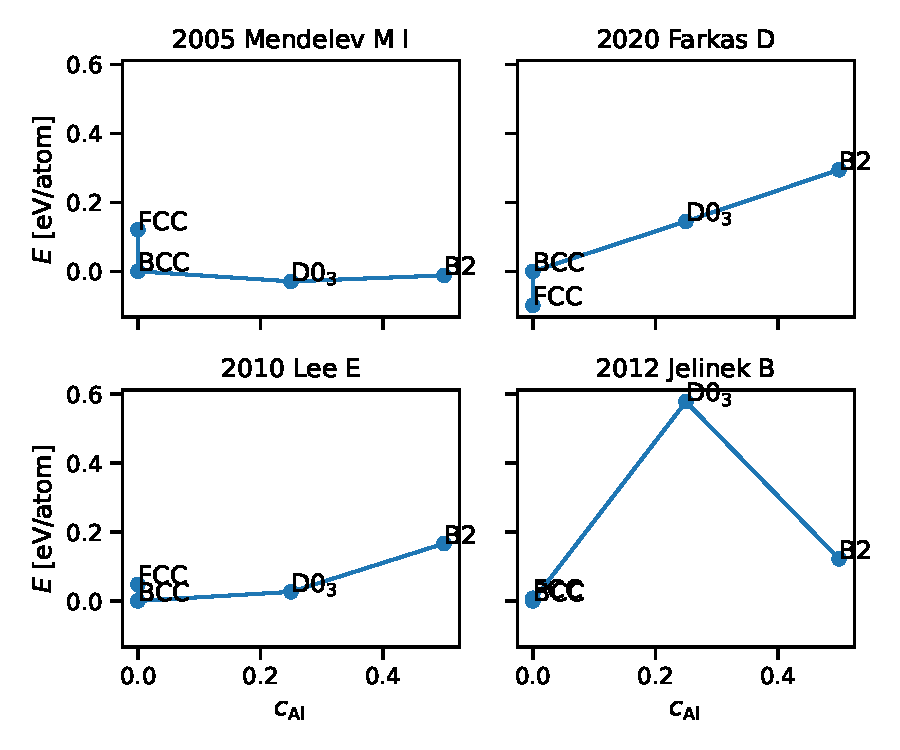
\includegraphics[width=\textwidth]{figures/zerok_phases}
    \caption{0K potential energy/atom for each of the relevant Fe-Al phases up to 50\% Al for several empirical potentials~\cite{mendelev2005effect, lee2010modified, jelinek2012modified, farkas2020model}.}
    \label{fig:0K_phases}
\end{figure}
%

For the two potentials that show promising results, we increase the level of complexity and consider the free energy of the phases in the simplifying limit of non-interacting defects and no vibrations -- i.e., we linearly extrapolate dilute point defect energies and include configurational entropy.
The calculation of the defect potential energy is simply the difference of the pristine and defected supercells.
For BCC this is easy, it is just a dilute Al solute.
Similarly, \BTWO is fairly straightforward as our antisite we can be an Al antisite on the Fe sublattice, or an Fe antisite on the Al sublattice.
For \DOTHREE things are slightly more complicated -- Fe antisites can exist on the Al sublattice, but Al antisites have a choice among two symmetry-unique Fe sublattices.
One of these Fe sublattices shares a simple-cubic sublattice with Al; this means it makes up only four of the 16 atoms in the \DOTHREE unit cell and has only other Fe atoms as first nearest neighbours.
The other sublattice is a simple cubic lattice occupied only by Fe atoms, which has four Al nearest neighbours and four Fe nearest neighbours.
We label the latter sublattice with a larger population ``aFe'', and the first, less populous sublattice ``bFe''.
The solute/antisite formation energies for all sublattices are shown in Table~\ref{tab:dilute}.
The most important feature here is the formation energy of Al in bulk BCC.
Since we know from experiment that the solubility of Al in Fe is quite large, and indeed at experimental conditions the system is observed to be (except for SRO) in a solid solution state, we can expect dilute Al to have a favourable formation energy.
This is the case for the potential of Mendelev \etal, but not that of Lee \etal.
%
% https://www.tablesgenerator.com/#
\begin{table}[]
    \centering
    \label{tab:dilute}
    \begin{tabular}{l|l|lll|ll}
                 & BCC   & \multicolumn{3}{l|}{D03} & \multicolumn{2}{l}{B2} \\
                 & form  & Al      & aFe   & bFe    & Al         & Fe        \\ \hline
        Mendelev & -0.31 & -0.07   & 0.71  & -0.22  & -0.38      & 1.79      \\
        Lee      & 0.24  & 0.03    & 1.03  & 0.67   & -0.50      & 1.75
    \end{tabular}
    \caption{Dilute formation energies (eV) for formation energy in the BCC and insertion of an antisite on the labeled sublattice. Results shown for the potentials of Mendelev \etal~\cite{mendelev2005effect} and Lee \etal~\cite{lee2010modified}. All values from zero-pressure minimizations and supercells size-converged to <0.001 eV.}
\end{table}

Under some sever simplifications, we can use these formation energies to generate a new phase diagram by linearly extrapolating the defect concentrations, shown in Fig.~\ref{fig:0K_dilute_phases} for 523 K.
Here we ignore the possibility of concentration-preserving antisite pairs and only allow deviation from the ideal structure by adding an antisite (i.e.~solute for BCC) which moves the composition in the appropriate direction.
For \DOTHREE a further simplification is made that the Fe sublattice with the more favourable potential energy of formation fills completely first, before the second sublattice starts to be occupied.
For the Mendelev potential this means the bFe sites become occupied before the aFe sites, i.e. we transition the system to a \BTWO ordering and then further Al antisites on the remaining simple cubic Fe sublattice (aFe for \DOTHREE).
In all cases configurational entropy comes from occupying the appropriate sublattice with fraction $s$ (i.e.~$s=1$ for solutes in BCC, $s=0.25$ for the \DOTHREE Al sublattice, etc.) with a defect concentration $c$: $S_\mathrm{mix} = -s k_B ((1 - \tilde{c}) \ln((1 - \tilde{c})) + \tilde{c}\ln\tilde{c})$, where $\tilde{c} = c/s$ so that entropy is maximized when the sublattice is half-occupied.
The phase diagram itself is not particularly meaningful for predicting phases across the composition range, for instance the assumption of non-interacting Al solutes in BCC certainly breaks down well before 50\% Al! However, it shows that the Mendelev potential favours the introduction of Al solutes into the BCC matrix, while for the Lee potential even the addition of configurational entropy is not enough to stabilize Al defects and the solubility remains very close to zero.
Thus, from here on we will focus only on the potental of Mendelev \etal~\cite{mendelev2005effect}.
%
\begin{figure}[h]
    \centering
    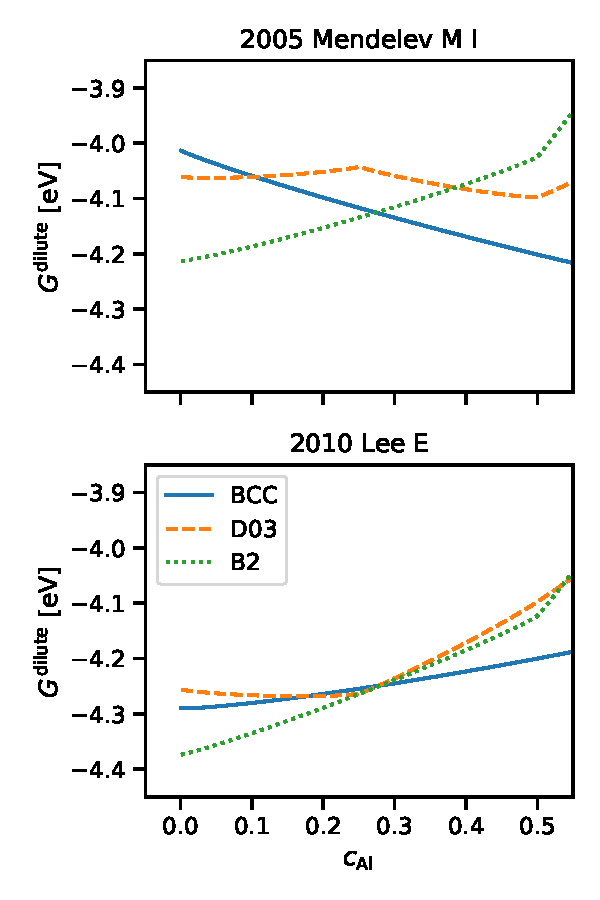
\includegraphics[width=0.8\textwidth]{figures/zerok_phases_dilute_point_defects}
    \caption{Phase diagram approximations at 523 K using linearly-extrapolated dilute defect formation energies and ideal entropy of mixing. Results shown for the potentials of Mendelev \etal~\cite{mendelev2005effect} and Lee \etal~\cite{lee2010modified}.}
    \label{fig:0K_dilute_phases}
\end{figure}
%

Next, in the region of experimental interest we will relax the approximation of non-interaction for defects in our BCC and \DOTHREE phases.
To accomplish this we use 432-atom supercells (i.e. $3\times3\times3$ repeats of the 16-atom cubic \DOTHREE unit cell) with random distributions of defects -- Al anywhere for BCC, and Fe on the Al sublattice for \DOTHREE.
This is repeated for different defect concentrations with a special focus in the regime where the total Al concentration is around the experimental value of $\approx 18\%$, and with ten (five) independent trials for the BCC (\DOTHREE) lattices.
The resulting potential energy curves can be seen in Fig.~\ref{fig:0K_interacting_potential}.
As expected, with sufficiently high Al concentrations, defect-defect interactions in the solid solution cause the potential energy to be concave-up.
Similarly, introducing Fe antisite defects to the \DOTHREE Al-sublattice is only favourable until a little more than one-fifth of these sites are occupied by an Fe atom. (20\% sublattice occupation equates to 5\% less Al concentration compared to ideal \DOTHREE since the sublattice makes up only a quarter of the system.)
%
\begin{figure}[h]
    \centering
    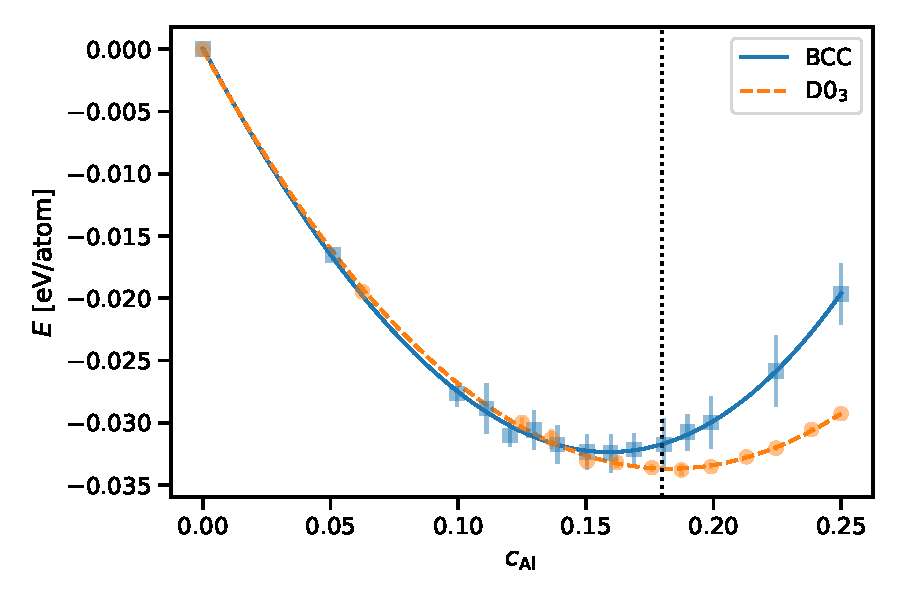
\includegraphics[width=\textwidth]{figures/zerok_interacting_defect_potential}
    \caption{Potential energy curves for finite concentrations of of defect (Al solutes for BCC, Fe antisite atoms on the Al sublattice for \DOTHREE). Values average over ten random configurations for each structure at each concentration, and standard deviations are shown as error bars (for \DOTHREE these are very small). The dashed black line indicates nominal experimental Al composition.}
    \label{fig:0K_interacting_potential}
\end{figure}
%

At 0K this potential actually gives the defected \DOTHREE structure as more preferable than a random solution, although as shown in Fig.~\ref{fig:0K_interacting_potential} this difference is extremely small.
While keeping all of the Al on the Al sublattice of the \DOTHREE structure is energetically favourable, it comes at an entropic cost.
As shown in Fig.~\ref{fig:0K_interacting_mixing}, this very small potential energy benefit is quickly washed out at finite temperatures.
In fact, even at the ideal \DOTHREE concentration of 25\% Al, the solid solution is preferable to \emph{pristine} \DOTHREE.
However, the \emph{defected} \DOTHREE (i.e.~with concentration-neutral antisite pairs) may still be more preferable according to this potential, but we did not study this scenario.
Distinguishing highly-defected \DOTHREE from solid solution would anyhow not be trivial, and in Fig.~\ref{fig:0K_interacting_potential} we can see that the potential energies of solid solution and \DOTHREE merge almost seamlessly below 15\% Al.
The key message from this data is that the potential of Mendelev \etal~does indeed predict solid solution Fe-Al at the experimental conditions, but the relative potential energy cost of \DOTHREE ordering is minimal (or even favourable) and so short-range-ordering (SRO) is very plausible.
%
\begin{figure}[h]
    \centering
    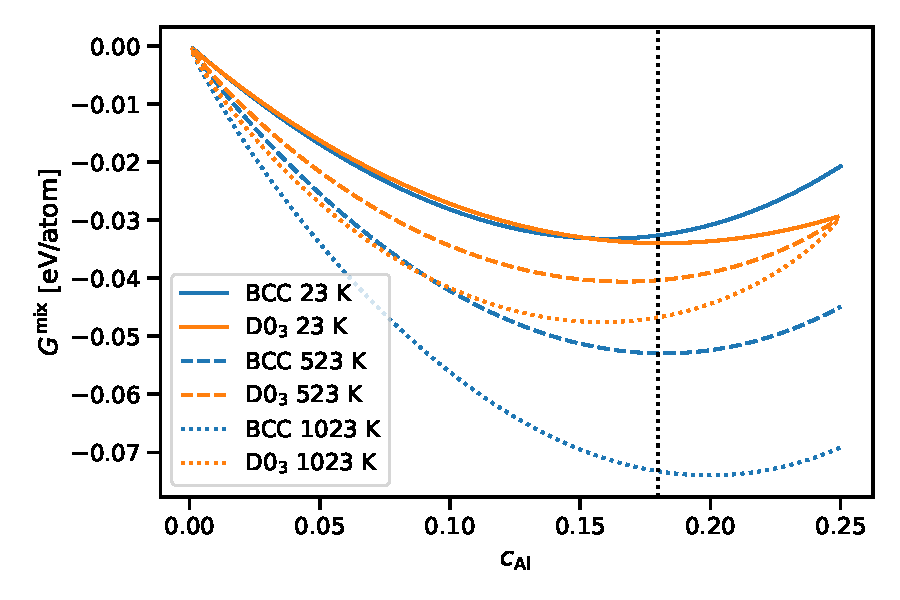
\includegraphics[width=\textwidth]{figures/zerok_interacting_defect_mixing}
    \caption{Phase formations at three temperatures for the BCC and \DOTHREE phases using entropy of mixing and fit curves for the potential energy of interacting Al solutes (Fe antisites on the Al sublattice) in the BCC (\DOTHREE) phase.}
    \label{fig:0K_interacting_mixing}
\end{figure}
%

As a final 0K exploration of SRO with this potential, we directly explore the cost of creating chemically ordered precipitates in the solid solution matrix.
Starting with a random solution of Al near the experimental concentration, we create a 1024-atom supercell and a corresponding reference supercell the same size with \DOTHREE or \BTWO ordering.
In the solid solution cell we begin converting the site occupation from random to that in the reference cell by always choosing a random first-nearest-neigbour (1NN) from among atoms already in the ``cluster''.
We repeat this process until one eighth of the atoms have been converted.
Since new atoms are selected for addition to the cluster by random choice from among available neighbours, any atom that is the 1NN of multiple atoms in the cluster has an increased chance to be chosen.
This promotes the growth of a cluster with a (statistically) smooth interface with the solid solution, but no further efforts were made to control the shapes of the clusters.
At each step the entire structure is minimized at zero pressure and the voronoi volumes of all atoms within the cluster are summed up to give an effective cluster volume, which is then converted to a radius under the assumption of a spherical shape.
The results of this process for both \DOTHREE and \BTWO are shown in Fig.~\ref{fig:0K_clusters}, repeated ten times for each lattice type with different initial solid solution distributions and different cluster growth.
In both cases there is a large variance across different trials, both show some routes for energetically favourable cluster formation, and both show an arithmetically averaged cluster energy that is much larger in magnitude than the thermal energy but comparable compared to point defects.
From this we conclude that this potential may plausibly show SRO in either \DOTHREE or \BTWO ordering in some local environments found in the 18\% solid solution, and more expensive finite-temperature studies are worthwhile.
One surprising observation is that the average cluster formation energy is actually \emph{more} favourable for \BTWO than \DOTHREE.
This is unexpected since referring back to Fig.~\ref{fig:0K_phases}, we can see that the pure 0K energy of \BTWO is actually slighlty higher than that of \DOTHREE.
One explanation for this is that the phases are simply very close in energy and our statistics are not sufficient to capture the preference for \DOTHREE.
Alternatively, it may simply be that the system is expressing a preference for ever more Al, as filling 1/8th of the supercell with \BTWO gives a higher overall Al concentration than filling it with \DOTHREE.
We will not examine this further directly since our main objective for these cluster calculations was to assess whether or not SRO would be plausible, and it is.
%
\begin{figure}[h]
    \centering
    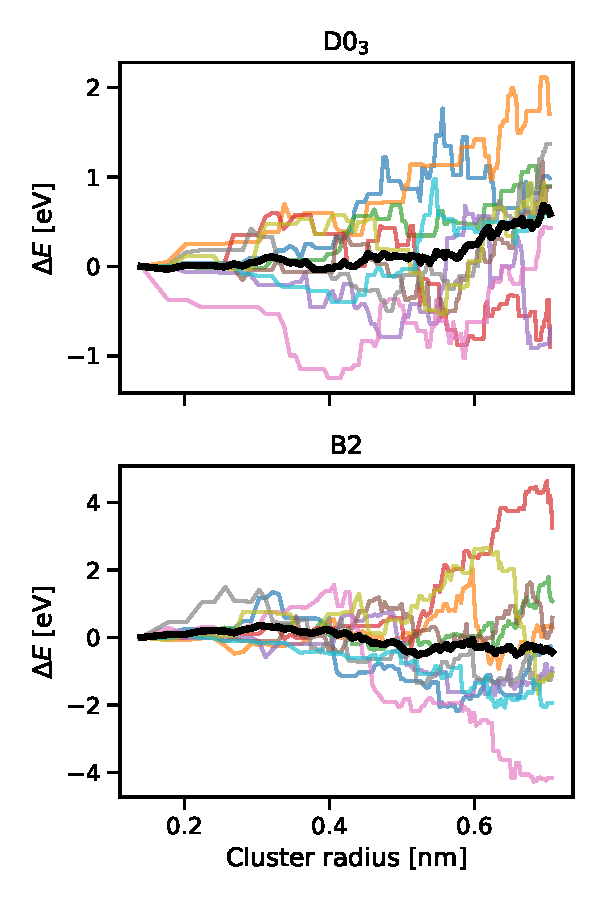
\includegraphics[width=0.8\textwidth]{figures/zerok_clusters}
    \caption{Potential energy as changes as a function of cluster volume by species-flipping random solid solutions to build pseudo-random clusters conforming to the occupation pattern of a reference secondary phase. Individual runs shown in colour with the arithmetic average shown thick and in black. See text for more detail.}
    \label{fig:0K_clusters}
\end{figure}
%

% TODO: add TILD calculations for pure phases as justification that vibrations won't ruin anything?